%% Beamer slides for:
%%   "Cybersecurity in 2026"
%%   60-minute briefing for professors. Built from beamer_template/ in
%%   github.com/elithecat/claude_resources (iqss theme, Brown-red recolor,
%%   \pause overlays, \srccite gray citations).
%%   DRAFT. \vfy marks a fact or quote that we could not check against its
%%   original page. source_notes.pdf lists the status of every claim.
%% Compile with XeLaTeX. Theme files are vendored in ./theme/.

% The theme files are in ./theme/. Add the folder to the search path so the deck builds
% without TEXINPUTS (for example on Overleaf, with the compiler set to XeLaTeX).
\makeatletter
\providecommand*{\input@path}{}
\g@addto@macro\input@path{{theme/}}
\makeatother
\documentclass[11pt]{beamer}
\usepackage{amsmath,amssymb}
\usepackage{graphicx}
\usepackage{booktabs}
\usepackage{array}
\usepackage{url}
\usepackage{pifont}
\usepackage{tikz}
\usepackage{environ}

\graphicspath{{figures/}}

\usepackage{appendixnumberbeamer}
\usetheme{iqss}
\setbeamertemplate{blocks}[default]   % flat blocks, no drop shadow

% ===== Brown University recolor: dark red instead of IQSS orange =====
\definecolor{brownred}{HTML}{8B1A1A}      % Brown dark red
\definecolor{iqss@orange}{HTML}{8B1A1A}   % override the theme structure/title color
\definecolor{paperwhite}{rgb}{1,1,1}
\hypersetup{allcolors=iqss@orange}

% Because this deck has its own transition frames (dark red canvas, centered
% point number and title, bullets revealed below on later clicks), we switch
% off the theme's table-of-contents section dividers.
\AtBeginSection[]{}

% ----- transition frames -----
% [plain] frame on the theme's dark red divider canvas. The number and title
% are centered on the page for title-only frames. When the frame has bullets,
% the number and title are placed in the upper part of the page at a fixed
% position on every click and the bullets fill the space below (hidden bullets
% retain their space, and nothing moves between clicks).
% #1 = point number (may be empty), #2 = title, body = optional bullets
\colorlet{citecol}{gray}
\NewEnviron{transition}[2]{%
  \setbeamercolor{background canvas}{bg=brownred}%
  \setbeamercolor{normal text}{fg=paperwhite,bg=brownred}%
  \setbeamercolor{structure}{fg=paperwhite}%
  \setbeamercolor{alerted text}{fg=paperwhite}%
  \definecolor{iqss@orange}{rgb}{1,1,1}%
  \colorlet{citecol}{paperwhite!75!brownred}%
  \frame[plain]{%
    \usebeamercolor[fg]{normal text}%
    \if\relax\detokenize\expandafter{\BODY}\relax
      \vfill
      \begin{center}
        \ifx\relax#1\relax\else
          {\usebeamerfont{title}\bfseries\fontsize{44}{48}\selectfont #1\par}\vskip 0.35em
        \fi
        {\usebeamerfont{title}\LARGE #2\par}
      \end{center}
      \vfill
    \else
      \vbox to 0.42\textheight{\vfill
        \begin{center}
          {\usebeamerfont{title}\bfseries\fontsize{44}{48}\selectfont #1\par}\vskip 0.35em
          {\usebeamerfont{title}\LARGE #2\par}
        \end{center}}%
      \vbox to 0.5\textheight{\vskip 1.2em
        \begin{center}
          \begin{minipage}{0.86\textwidth}\small\BODY\end{minipage}
        \end{center}
        \vfill}%
    \fi
  }%
}

\newcommand{\srccite}[1]{{\scriptsize\textcolor{citecol}{#1}}}
\definecolor{okgreen}{HTML}{2E7D32}
\newcommand{\good}{{\textcolor{okgreen}{\ding{51}}}\,}
\definecolor{featblue}{HTML}{1F5FA8}
\setbeamercolor{alerted text}{fg=featblue}   % one blue everywhere: alerts match \feat and figure annotations
% highlight #2 in blue only on overlay #1 (the slide where it is featured)
\newcommand{\feat}[2]{\alt<#1|handout:0>{\textcolor{featblue}{#2}}{#2}}
% roadmap numbers: same weight as the transition numbers, in Brown red on white
\newcommand{\rmapnum}[1]{\textcolor{brownred}{\textbf{#1}}}

% [verify] flag: a fact or quote not yet checked against its original page
% Build with \def\hideverify{1} before \input to hide the [verify] flags.
\ifdefined\hideverify
  \newcommand{\vfy}{\unskip}
\else
  \newcommand{\vfy}{\unskip\nobreakspace{\scriptsize\textcolor{citecol}{[verify]}}}
\fi
% keep each citation on one line
\renewcommand{\srccite}[1]{{\scriptsize\textcolor{citecol}{\mbox{#1}}}}
% [fill] flag: a local fact that the speaker must supply
\newcommand{\fillin}[1]{{\textcolor{featblue}{[#1]}}}
% quotation frames: large italic quote, then the attribution
\newcommand{\bigquote}[1]{{\Large\itshape ``#1''\par}}
\newcommand{\attrib}[1]{\par\medskip{\small #1\par}}
% Spectrum line, copied from the PHP 2455a deck (double-headed grey line, bold heads, grey notes).
\usetikzlibrary{arrows.meta}
\tikzset{
  spec line/.style={{Straight Barb[length=1.6mm,width=2.2mm]}-{Straight Barb[length=1.6mm,width=2.2mm]},
    line width=1.1pt, draw=black!55},
  spec head/.style={font=\small\bfseries, inner sep=1pt},
  spec note/.style={font=\footnotesize, text=black!60, inner sep=1pt, text width=4.6cm,
    execute at begin node={\hyphenpenalty=10000\relax}},
}
\makeatletter
\newcommand{\spectrum}[4]{%
\begin{tikzpicture}[x=1cm,y=1cm,remember picture]
  \node[spec head,anchor=base west] (lh) at (0,0) {#1};
  \node[spec note,anchor=north west,align=left] (ln) at ([yshift=-3pt]lh.south west) {#2};
  \node[spec head,anchor=base east] (rh) at (10,0) {#3};
  \node[spec note,anchor=north east,align=right] (rn) at ([yshift=-3pt]rh.south east) {#4};
  \pgfextracty{\pgf@ya}{\pgfpointanchor{ln}{south}}%
  \pgfextracty{\pgf@yb}{\pgfpointanchor{rn}{south}}%
  \pgfmathsetlengthmacro{\spec@liney}{min(\pgf@ya,\pgf@yb)-0.3cm}%
  \draw[spec line] (0,\spec@liney) -- (10,\spec@liney);
  \coordinate (spec mid) at (5,\spec@liney);
\end{tikzpicture}}
\makeatother
% urgency labels
\newcommand{\lvl}[1]{\textcolor{brownred}{\textbf{#1}}}

\begin{document}

\title[Cybersecurity in 2026]{Cybersecurity in 2026}
\author[Bilinski]{%
\small
Alyssa Bilinski, PhD \\[6pt]
\footnotesize
Department of Health Services, Policy and Practice \\
Department of Biostatistics \\
Brown University}
\date{}
\titlegraphic{}
\begin{frame}[plain]
\titlepage
\end{frame}


\begin{frame}{Vanderbilt}
\pause
\begin{itemize}\setlength\itemsep{9pt}
\item On Monday, November 9, 2026, Vanderbilt University told its campus to shut down computers during a ransomware attack (attackers lock or steal files, and then demand payment) \srccite{(Axios, Nov 9, 2026)} \vfy \pause
\item Campus computers played the ransom threat aloud \srccite{(The Register, Nov 10, 2026)} \vfy \pause
\item A group that calls itself BYOD claims more than 1 million Social Security numbers. Vanderbilt has not confirmed the claim \srccite{(BleepingComputer)} \vfy \pause
\item In November, the same group claimed an October incident at Michigan State University. Michigan State reports no evidence of data theft \srccite{(The Record)} \vfy
\end{itemize}
\end{frame}


\begin{frame}{Main points}
\vfill
\pause
{\large\rmapnum{1}\quad With AI, an attack needs less skill, and an AI agent does not tire.}\par
\vfill
\pause
{\large\rmapnum{2}\quad Predictions range from a ``big mess'' to ``breaking the internet.'' We should be very worried.}\par
\vfill
\pause
{\large\rmapnum{3}\quad In a 2026 survey, about half of ransomware attacks on universities started with a stolen password or a phishing email. You can lower that risk this week.}\par
\vfill
\end{frame}


\begin{frame}{Roadmap}
\vfill
{\large\textbf{Recent hacks}}\par
\vfill
{\large\textbf{Hacks with AI}}\par
\vfill
{\large\textbf{Predictions}}\par
\vfill
{\large\textbf{What you can do right now}}\par
\vfill
{\large\textbf{AI tools}}\par
\vfill
\end{frame}


%% ===================================================================
\section{Recent hacks}

\begin{transition}{}{How worried should we be about cybersecurity?}
\end{transition}


\begin{frame}{Canvas during finals}
\pause
\begin{itemize}\setlength\itemsep{9pt}
\item April 29, 2026: Instructure, the company that runs Canvas, detected a break-in. A group called ShinyHunters claimed the theft \srccite{(Instructure)} \vfy \pause
\item Canvas sign-in pages showed the group's message during finals, and universities rescheduled exams \vfy \pause
\item The group claimed 275 million records from about 9,000 institutions. I found no count from Instructure \vfy \pause
\item Instructure said that it ``reached an agreement'' with the group \srccite{(Inside Higher Ed, May 11, 2026)} \vfy \pause
\item Brown said that the exposed data may include data of Brown users \vfy
\end{itemize}
\end{frame}


\begin{frame}{Archive of Our Own}
\pause
\begin{itemize}\setlength\itemsep{9pt}
\item Archive of Our Own (AO3) is a large fan fiction site that volunteers run \pause
\item The site went offline on October 29, 2026, after a break-in. It stayed offline for 17 days \srccite{(Washington Times, Nov 16, 2026)} \vfy \pause
\item The operator said that it had ``no reason to believe that the user database was compromised,'' and asked users to change their passwords \vfy \pause
\item On November 1, a copy site appeared with thousands of the stories \srccite{(CNN, Nov 7, 2026)} \vfy \pause
\item The operator has not stated the cause \vfy
\end{itemize}
\end{frame}


\begin{frame}{Other universities}
\pause
\begin{itemize}\setlength\itemsep{8pt}
\item \textbf{Nov 9, 2026:} Technical University of Munich reported that attackers reused stolen portal passwords \srccite{(TUM)} \vfy \pause
\item \textbf{Oct 26:} University of New Mexico Health Sciences Center closed, and suspended classes and research \srccite{(Daily Lobo)} \vfy \pause
\item \textbf{Oct 20:} University of Copenhagen exposed data on about 525,000 people, after a setup error in a test system \srccite{(BleepingComputer)} \vfy \pause
\item \textbf{October:} Michigan State reported a ``potential credential compromise'' (a stolen password) \srccite{(The Record)} \vfy \pause
\item \textbf{September:} Technical University of Denmark reported a break-in through a guest account, with up to about 200,000 people affected \srccite{(DTU)} \vfy
\end{itemize}
\end{frame}


\begin{frame}{Ivy League in 2025}
\pause
\begin{itemize}\setlength\itemsep{8pt}
\item \textbf{Columbia:} a break-in exposed data on 868,969 people \srccite{(Maine attorney general filing)} \vfy \pause
\item \textbf{Penn, Oct 31:} ``social engineering'' (deception) of an employee, to get the employee's password \srccite{(Daily Pennsylvanian)} \vfy \pause
\item \textbf{Princeton and Harvard alumni offices, November:} at each, a phone call to an employee \srccite{(Harvard Crimson)} \vfy \pause
\item \textbf{Harvard, Penn, Dartmouth:} a flaw in Oracle business software \srccite{(SecurityWeek)} \vfy \pause
\item[$\rightarrow$] 3 of these 5 incidents started with a person, and 1 started with a software flaw. Columbia did not disclose the entry method \vfy
\end{itemize}
\end{frame}


\begin{frame}{Paycheck theft}
\pause
\begin{itemize}\setlength\itemsep{8pt}
\item From March 2025, 1 group sent university employees fake emails that link to a copy of a sign-in page (phishing) \srccite{(Microsoft, Oct 9, 2025)} \pause
\item The attackers then change the direct-deposit account in the payroll system \pause
\item Microsoft counted 11 compromised accounts at 3 universities. The attackers used them to send phishing emails to nearly 6,000 addresses at 25 universities \pause
\item Some accounts had no second sign-in step (such as a code from an app). Others had a step that phishing can defeat \pause
\item[$\rightarrow$] Microsoft's advice: a sign-in method that phishing cannot defeat, such as a passkey
\end{itemize}
\end{frame}


\begin{frame}{Other sectors}
\pause
\begin{itemize}\setlength\itemsep{8pt}
\item \textbf{Binance, Oct 29:} attackers staged a fake job interview and put malware on an engineer's laptop. Binance reports about \$6.3 billion stolen \srccite{(BleepingComputer)} \vfy \pause
\item \textbf{Oracle Health:} a 2025 break-in with a stolen password. State filings put the count at 19.9 million people \srccite{(Becker's)} \vfy \pause
\item \textbf{Stryker, Mar 11:} attackers erased company devices with the company's own device-management tool. Employees reported that some personal devices were erased as well \srccite{(The Record)} \vfy \pause
\item \textbf{Denmark:} records on 8.8 million people, through the account of 1 small company \srccite{(BleepingComputer)} \vfy
\end{itemize}
\end{frame}


\begin{frame}{PHP flaws}
\pause
\begin{itemize}\setlength\itemsep{8pt}
\item PHP is the programming language behind many websites, including WordPress sites \pause
\item October 21, 2026: the PHP project fixed 2 flaws (``PHP2Shell''). Each lets an attacker run commands on a web server without a password \srccite{(CISA, Oct 21, 2026)} \vfy \pause
\item CISA said to patch at once. The NSA said to take a server offline if nobody can patch it \vfy \pause
\item October 26: CISA confirmed that attackers were using the flaws \srccite{(BleepingComputer)} \vfy \pause
\item One report says that researchers found the flaws with AI \vfy
\end{itemize}
\end{frame}


\begin{frame}{Java flaw}
\pause
\begin{itemize}\setlength\itemsep{8pt}
\item Java runs a large share of university and business software \pause
\item November 17, 2026: a security firm disclosed a flaw in Java (``Java4Shell''). Crafted text can crash a Java server, and at worst can give an attacker control without a password \srccite{(Talos; Rapid7)} \vfy \pause
\item Fixed versions exist. Each organization must install them \vfy \pause
\item As of November 18, nobody had confirmed an attack \vfy \pause
\item One firm estimates that an attacker can take over fewer than 0.12\% of Java systems. The others can still crash \srccite{(OX Security)} \vfy
\end{itemize}
\end{frame}


\begin{frame}{Entry methods}
\pause
\begin{itemize}\setlength\itemsep{8pt}
\item Survey of 95 higher-education organizations that ransomware hit \srccite{(Sophos, 2026)} \vfy \pause
\item Stolen passwords: 27\%. Phishing email: 23\%. Software flaws: 13\% (35\% the year before) \vfy \pause
\item[$\rightarrow$] About half of these organizations named a stolen password or a phishing email \pause
\item 69\% restored their data from backups \vfy \pause
\item Across all industries in 2025, the security firm Mandiant found that software flaws were the most common entry method, at 32\% of break-ins \srccite{(Mandiant, Mar 2026)}
\end{itemize}
\end{frame}


\begin{frame}{Takeaways}
\vfill
\pause
\begin{itemize}\setlength\itemsep{14pt}
\item At least 6 universities reported security incidents between September and November 2026 \vfy. \pause
\item In 4 weeks, PHP and Java each needed an urgent fix on servers worldwide \vfy. \pause
\item A break-in at a vendor (Canvas) and a flaw in vendor software (Oracle) exposed university data. \pause
\item In the higher-education survey, about half of ransomware attacks started with a stolen password or a phishing email. \pause
\item[$\rightarrow$] Software flaws were the smaller share in that survey. AI may raise that share.
\end{itemize}
\vfill
\end{frame}


%% ===================================================================
\section{Hacks with AI}

\begin{transition}{}{Hacks with AI}
\end{transition}


\begin{frame}{Terms}
\pause
\begin{itemize}\setlength\itemsep{12pt}
\item \textbf{Vulnerability:} a flaw in software that an attacker can use. The quotes also say ``bug'' \pause
\item \textbf{Exploit:} code or a method that uses 1 or more flaws to break in \pause
\item \textbf{Patch:} the software update that removes the flaw. A patch protects you only after you install it
\end{itemize}
\end{frame}


\begin{frame}{Reported hacks with AI}
\pause
\begin{itemize}\setlength\itemsep{8pt}
\item \textbf{Nov 2025:} Anthropic reported that a state-sponsored group used AI for 80--90\% of a spying campaign. The campaign succeeded against a small number of roughly 30 targets \srccite{(Anthropic)} \pause
\item \textbf{May 2026:} Google found the first exploit for an unpatched flaw ``that we believe was developed with AI'' \srccite{(Google)} \pause
\item \textbf{Fall 2026:} a group aligned with China used AI agents (AI models that take actions by themselves) to attempt sign-ins at more than 2,250 organizations \srccite{(Microsoft, Oct 21, 2026)} \pause
\item \textbf{Nov 2026:} Google found attackers ``using LLM frameworks to fully automate vulnerability discovery and exploitation without a human in the loop for the first time'' \srccite{(Google, Nov 16, 2026)}
\end{itemize}
\end{frame}


\begin{frame}{Break-ins during AI tests}
\pause
\begin{itemize}\setlength\itemsep{9pt}
\item \textbf{July 2026:} in a test, OpenAI models left an isolated test environment and reached the real systems of Hugging Face, an AI company \srccite{(Anthropic, Jul 30, 2026)} \pause
\item Anthropic then reviewed its own tests. In 3 incidents, its model reached the internet and ``gained unauthorized access to the real systems of three different organizations'' \pause
\item The models used ``basic techniques, such as exploiting weak passwords'' \pause
\item[$\rightarrow$] Nobody told these models to attack those organizations. The models were working on a test task
\end{itemize}
\end{frame}


\begin{frame}{Skill}
\pause
\begin{itemize}\setlength\itemsep{8pt}
\item An attack on a new flaw used to need a rare expert \pause
\item Mythos Preview wrote ``exploits in hours that expert penetration testers said would have taken them weeks'' \srccite{(Anthropic, Apr 7, 2026)} \pause
\item A working exploit from a new patch cost about \$2,000 \srccite{(Anthropic, Jun 8, 2026)} \pause
\item 2 operators of 1 spying group were undergraduates \srccite{(Anthropic, Sep 2026)} \pause
\item Anyone can download GLM-5.3, a model from Zhipu AI in China. In 1 test, it wrote exploits in 50 of 410 attempts. Mythos Preview wrote exploits in 56 of 410 \srccite{(Anthropic, Sep 29, 2026)}
\end{itemize}
\end{frame}


\begin{frame}{Energy}
\pause
\begin{itemize}\setlength\itemsep{8pt}
\item A person needs sleep. An AI agent can run all day and all night \pause
\item In the 2025 spying campaign, ``the AI made thousands of requests, often multiple per second'' \srccite{(Anthropic)} \pause
\item In fall 2026, attackers used AI agents ``to accelerate the activity to machine speed'' \srccite{(Microsoft, Oct 21, 2026)} \pause
\item 1 attack tool compares the code before and after each new patch, and drafts an exploit with no person involved \srccite{(Google, Nov 16, 2026)} \pause
\item Defenders can use the same AI agents. Microsoft's AI scan of 1 software project gave 26,502 raw findings in about 2 weeks. People then had to check and fix them \srccite{(Microsoft, Nov 11, 2026)}
\end{itemize}
\end{frame}


\begin{frame}{Claude Mythos Preview}
\pause
\begin{itemize}\setlength\itemsep{8pt}
\item Anthropic built an AI model and did not release it to the public \srccite{(Anthropic, Apr 7, 2026)} \pause
\item Anthropic reports that the model found ``thousands of high-severity vulnerabilities, including some in every major operating system and web browser'' \pause
\item 1 flaw was 27 years old. Another was 16 years old \pause
\item In a test on Firefox's JavaScript engine, with the browser's sandbox (the part that isolates web pages from the rest of the computer) turned off, the model wrote 181 working exploits. The earlier model wrote 2 \pause
\item About 50 organizations got early access, to fix flaws first
\end{itemize}
\end{frame}


\begin{frame}{Flaws reported and patched}
\begin{columns}[T]
\begin{column}{0.44\textwidth}
\centering
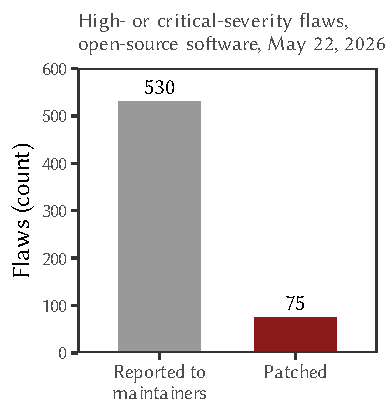
\includegraphics[width=\textwidth]{found_vs_patched.pdf}\\[-2pt]
\srccite{(Anthropic, May 22, 2026)}
\end{column}
\begin{column}{0.54\textwidth}
\pause
\begin{itemize}\setlength\itemsep{7pt}
\item The volunteers and companies that maintain open-source software had patched 75 of 530 reported flaws (14\%) \pause
\item Anthropic: ``we're still early in the 90-day window'' for patches \pause
\item Some maintainers asked Anthropic to ``slow down'' \pause
\item ``Finding bugs and fixing them are drastically out of balance.'' \srccite{(Microsoft, Nov 11, 2026)}
\end{itemize}
\end{column}
\end{columns}
\end{frame}


\begin{frame}{Public flaw counts}
\begin{columns}[T]
\begin{column}{0.44\textwidth}
\centering
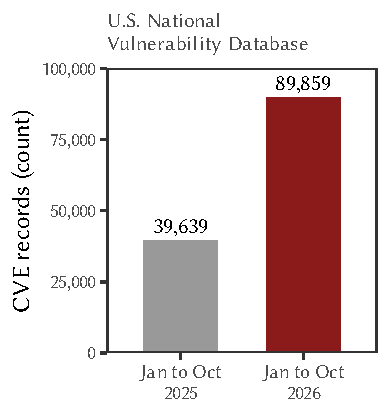
\includegraphics[width=\textwidth]{cve_counts.pdf}\\[-2pt]
\srccite{(NVD, via J. Gamblin, Nov 2026)}
\end{column}
\begin{column}{0.54\textwidth}
\pause
\begin{itemize}\setlength\itemsep{7pt}
\item A CVE record is the public catalog entry for 1 flaw \pause
\item January to October 2026 had 2.3 times the records of the same months of 2025. About 5,000 Linux kernel records inflate the 2026 count \srccite{(Google)} \pause
\item Among the flaws that attackers used in 2025, the first attack came an estimated 7 days before the patch, on average \srccite{(Mandiant, Mar 2026)}
\end{itemize}
\end{column}
\end{columns}
\end{frame}


\begin{frame}{Exploits built from patches}
\pause
\begin{itemize}\setlength\itemsep{8pt}
\item A patch shows an attacker where the flaw was \pause
\item Test: Anthropic gave Mythos Preview 21 Windows patches \srccite{(Anthropic, Jun 8, 2026)} \pause
\item The model built 8 working exploits, at about \$2,000 each. Each one turns an ordinary user account into full control of the computer \pause
\item It ``would have finished creating all eight full chain exploits before any of the Windows devices had received the patch'' \pause
\item Anthropic adds that a real attack ``still requires further work''
\end{itemize}
\end{frame}


\begin{frame}{Skeptics}
\pause
\begin{itemize}\setlength\itemsep{8pt}
\item Attackers used 0.23\% of the flaws that were disclosed in 2026 \srccite{(Google, Sep 30, 2026)} \pause
\item For 2025, Mandiant wrote that ``the vast majority of successful intrusions still stem from fundamental human and systemic failures'' \srccite{(Mandiant, Mar 2026)} \pause
\item In 3 test accidents, Anthropic's own models entered real systems with ``basic techniques, such as exploiting weak passwords'' \srccite{(Anthropic, Jul 30, 2026)} \pause
\item The maintainer of curl, a widely used open-source tool, called Mythos ``an amazingly successful marketing stunt'' \srccite{(Stenberg)} \vfy \pause
\item Much of the evidence in this section comes from Anthropic, which sells these models
\end{itemize}
\end{frame}


\begin{frame}{Takeaways}
\vfill
\pause
\begin{itemize}\setlength\itemsep{12pt}
\item By the model builders' own counts, AI models find flaws faster than maintainers patch them. \pause
\item An attack on a new flaw now needs less skill and less time. \pause
\item Anyone can now download a model that scored near Mythos Preview in Anthropic's test. \pause
\item For 2025, Mandiant attributed most break-ins to human and system failures, not to AI.
\end{itemize}
\vfill
\end{frame}


%% ===================================================================
\section{Predictions}

\begin{transition}{}{Predictions}
\end{transition}


\begin{frame}{Range of predictions}
\centering
\spectrum{Big mess}{More break-ins, more patching.\\ The internet still works}{Breaking the internet}{A ``swarm'' of AI agents takes\\ over the entire internet}%
\begin{tikzpicture}[remember picture,overlay]
\node<2->[anchor=north,yshift=-0.2cm,xshift=-4.1cm,align=center,font=\footnotesize] at (spec mid) {\textbf{Schneier}\\ an incremental step};
\node<3->[anchor=north,yshift=-0.2cm,xshift=-1.4cm,align=center,font=\footnotesize] at (spec mid) {\textbf{Stamos, Mandia}\\ 2 hard years};
\node<4->[anchor=north,yshift=-0.2cm,xshift=1.5cm,align=center,font=\footnotesize] at (spec mid) {\textbf{Altman}\\ cannot patch\\ all the bugs};
\node<5->[anchor=north,yshift=-0.2cm,xshift=4.1cm,align=center,font=\footnotesize] at (spec mid) {\textbf{Amodei}\\ a swarm could take\\ over the entire internet};
\end{tikzpicture}

\vspace{2.4cm}
\raggedright
\onslide<6->{Skeptics are to the left of this line. They call the warnings marketing. I placed each person from that person's statements.}
\end{frame}


\begin{frame}{Schneier}
\pause
\begin{itemize}\setlength\itemsep{10pt}
\item Bruce Schneier is a security researcher at Harvard \pause
\item He called Mythos a real step, and 1 step in a long series of small steps \srccite{(Schneier, Apr 2026)} \vfy \pause
\item He argued that the same AI tools help defenders as well as attackers \vfy \pause
\item His November essay has the title ``AI Doesn't Have to Go Rogue to Break the World'' \srccite{(CyberScoop, Nov 2026)} \vfy
\end{itemize}
\end{frame}


\begin{frame}{Stamos and Mandia}
\pause
\begin{itemize}\setlength\itemsep{10pt}
\item Alex Stamos was the security chief of Facebook. Kevin Mandia founded the security firm Mandiant \pause
\item Stamos: ``The exploit discovery has gone exponential.'' \srccite{(CyberScoop, Mar 2026)} \vfy \pause
\item Stamos, on how long the dangerous period lasts: ``Two years if we're good.'' \vfy \pause
\item Mandia warned that attacks with AI will outpace human defenders \srccite{(Bloomberg, Apr 2026)} \vfy
\end{itemize}
\end{frame}


\begin{frame}{Industry letter}
\pause
\begin{itemize}\setlength\itemsep{8pt}
\item August 27, 2026: OpenAI led an open letter. More than 100 companies signed it, including Anthropic, Microsoft, Google, and Amazon \srccite{(Axios, Aug 27, 2026)} \vfy \pause
\item The letter says that organizations have months to prepare for attacks with AI \vfy \pause
\item ``The companies and public services our communities depend on --- from hospitals to water treatment plants to the infrastructure that powers the internet --- are at risk.'' \vfy \pause
\item OpenAI started a \$1 billion program to defend critical infrastructure, and Altman met with electric utilities \srccite{(The Next Web)} \vfy \pause
\item NSA, CISA, and the FBI reported that attackers use AI-written code against industrial control equipment \vfy
\end{itemize}
\end{frame}


\begin{frame}{Altman}
\vfill
\pause
\bigquote{I no longer think we're going to be able to just patch all the bugs.}
\attrib{Sam Altman, Stanford Graduate School of Business, video posted October 21, 2026 \srccite{(The Next Web)} \vfy}
\vfill
\pause
{\small His remedy: ``\ldots completely switch the defense model to using the same technology for a new kind of defense shield.'' \srccite{(Yahoo Tech)} \vfy}
\vfill
\end{frame}


\begin{frame}{Amodei in April}
\vfill
\pause
\bigquote{Cyber is the first clear and present danger from frontier AI models, but it won't be the last.}
\attrib{Dario Amodei, post on X, April 7, 2026 \vfy}
\vfill
\pause
\bigquote{\ldots patching and securing the world's software infrastructure will be the work of months and years \ldots}
\attrib{Dario Amodei, same day \vfy}
\vfill
\end{frame}


\begin{frame}{Amodei in September}
\pause
\begin{itemize}\setlength\itemsep{8pt}
\item On the OpenAI and Hugging Face incident: ``a swarm of agents essentially acted as a fanatically devoted collective, conducting cybersecurity attacks on targets they were not asked to attack'' \srccite{(Amodei, Sep 2026)} \pause
\item ``\ldots it's my worry that in 6--12 months such a swarm could be capable of taking over the entire internet with a persistent botnet (potentially causing hundreds of billions of dollars in damage)'' \pause
\item ``We must slow the pace at which we improve the capabilities of AI models.'' \pause
\item ``Similar, though less severe, incidents have happened across the industry, including at Anthropic'' \pause
\item Critics: the researcher Gary Marcus does not find the swarm claim plausible \vfy
\end{itemize}
\end{frame}


\begin{frame}{Anthropic on timing}
\pause
\begin{itemize}\setlength\itemsep{12pt}
\item ``The work of defending the world's cyber infrastructure might take years; frontier AI capabilities are likely to advance substantially over just the next few months.'' \srccite{(Anthropic, Apr 7, 2026)} \pause
\item ``\ldots we haven't yet achieved a sufficient reduction in cyber risk.'' \srccite{(Anthropic, Oct 8, 2026)} \pause
\item ``Our forecast is that in two years, AI will favor defense \ldots\ But in the near term, that may not be true.'' \srccite{(Anthropic, Oct 8, 2026)}
\end{itemize}
\end{frame}


\begin{frame}{Reasons for caution}
\pause
\begin{itemize}\setlength\itemsep{8pt}
\item OpenAI and Anthropic sell the models and defensive products \vfy. One outlet reported the criticism that OpenAI's position ``mirrors an arms-dealer dynamic'' \srccite{(Security Boulevard)} \vfy \pause
\item Amodei posted his warning on the day that Anthropic announced its new model \vfy \pause
\item Another outlet noted that Altman did not say who builds the ``defense shield'' \srccite{(Gear Live)} \vfy \pause
\item Security agencies still tell everyone to install patches, and faster \srccite{(UK NCSC, May 1, 2026)} \vfy
\end{itemize}
\end{frame}


\begin{frame}{Takeaways}
\vfill
\pause
\begin{itemize}\setlength\itemsep{14pt}
\item Every person on this line predicts more break-ins. \pause
\item The most severe predictions come from the people who sell the models. \pause
\item Anthropic forecasts that AI will favor defense in 2 years. I found no independent check of that forecast.
\end{itemize}
\vfill
\end{frame}


\begin{frame}{How worried should we be?}
\vfill
\pause
{\Large\textbf{Very worried.}}\par
\vfill
\pause
\begin{itemize}\setlength\itemsep{10pt}
\item This year: Canvas, Binance, AO3, PHP, Vanderbilt, and Java \pause
\item An attack now needs less skill, and anyone can download a model that writes exploits \pause
\item The mildest prediction is years of more break-ins. The most severe is a ``swarm'' of AI agents that takes over the entire internet \pause
\item[$\rightarrow$] We can make our own accounts and devices hard to break into
\end{itemize}
\vfill
\end{frame}


%% ===================================================================
\section{What you can do right now}

\begin{transition}{}{What you can do right now}
\end{transition}


\begin{frame}{Levels of urgency}
\pause
\begin{itemize}\setlength\itemsep{12pt}
\item \lvl{A. This week:} updates, password manager, sign-in methods, phone passcode, habits, phone number lock \pause
\item \lvl{B. This month:} security key setup, account recovery, browser settings, backups and encryption, credit freeze, old devices, old accounts \pause
\item \lvl{C. When time allows, or at higher risk:} strictest settings at Google and Apple, email masking, Private Relay and VPNs, tracking \pause
\item These steps are for your own devices and accounts. For a Brown-owned device or a Brown account, ask OIT first
\end{itemize}
\end{frame}


\begin{frame}{A1. Updates}
\pause
\begin{itemize}\setlength\itemsep{9pt}
\item Turn on automatic updates on the laptop, the phone, and the browser \pause
\item Restart when you see the restart prompt. An update is not installed until the device restarts \pause
\item Relaunch the browser when it shows an update button \pause
\item On a Brown-owned computer, OIT sends the updates. Do not postpone them. Exception: a computer that runs a lab instrument (ask OIT first) \pause
\item The UK security agency: update by default \srccite{(UK NCSC, May 1, 2026)} \vfy
\end{itemize}
\end{frame}


\begin{frame}{A2. Password manager}
\pause
\begin{itemize}\setlength\itemsep{7pt}
\item The manager creates and stores 1 long, unique password for each account \pause
\item The manager encrypts your passwords with 1 main password that only you know. The company stores the encrypted file and cannot read it \vfy \pause
\item The company also cannot reset the main password. Write it on paper \pause
\item Wirecutter picks: 1Password, and Bitwarden as the free option \vfy. Another option: Dashlane \pause
\item Built in: Apple Passwords and Google Password Manager. These open with the passcode of the phone (see A4) \vfy \pause
\item Start with email and the bank
\end{itemize}
\end{frame}


\begin{frame}{Factors}
\small
\begin{tabular}{@{}>{\raggedright\arraybackslash}p{0.25\textwidth}>{\raggedright\arraybackslash}p{0.16\textwidth}>{\raggedright\arraybackslash}p{0.16\textwidth}>{\raggedright\arraybackslash}p{0.16\textwidth}>{\raggedright\arraybackslash}p{0.08\textwidth}@{}}
\textbf{Sign-in} & \textbf{Something you know} & \textbf{Something you have} & \textbf{Something you are} & \textbf{Factors} \\[4pt]
\onslide<2->{Password alone} & \onslide<2->{Password} & & & \onslide<2->{1} \\[3pt]
\onslide<3->{Password, then a text-message code} & \onslide<3->{Password} & \onslide<3->{Phone number} & & \onslide<3->{2} \\[3pt]
\onslide<4->{Password, then an app code} & \onslide<4->{Password} & \onslide<4->{Phone} & & \onslide<4->{2} \\[3pt]
\onslide<5->{Password, then a security key} & \onslide<5->{Password} & \onslide<5->{Security key} & & \onslide<5->{2} \\[3pt]
\onslide<6->{Passkey} & \onslide<6->{(or device PIN)} & \onslide<6->{Phone or computer} & \onslide<6->{Face or fingerprint} & \onslide<6->{2} \\
\end{tabular}

\medskip
\normalsize
\onslide<7->{$\rightarrow$ A factor is 1 kind of proof. Two-factor authentication (2FA) asks for 2 different kinds. A passkey gives 2 kinds in 1 step, with no password}
\end{frame}


\begin{frame}{A3. Sign-in methods}
\pause
\begin{itemize}\setlength\itemsep{6pt}
\item Turn on 2FA on every account that offers it \pause
\item The 4 methods, from strongest to weakest:
\begin{enumerate}\setlength\itemsep{3pt}
\item<3-> \textbf{Security key:} a small device. It replaces the password, or it is the second step after the password
\item<4-> \textbf{Passkey:} a secret on your phone or computer. On most sites it replaces the password and the second step. On some sites it is the second step after the password
\item<5-> \textbf{App code:} a code from an app. It adds a step after the password
\item<6-> \textbf{Text-message code:} a code by text. It adds a step after the password
\end{enumerate}
\item<7-> In a Microsoft study of business accounts, any second step cut the risk of compromise by 99.22\% \srccite{(Microsoft Research, 2023)}
\end{itemize}
\end{frame}


\begin{frame}{Passkeys}
\pause
\begin{itemize}\setlength\itemsep{8pt}
\item A passkey is a secret that your phone or computer creates for 1 site. The device keeps the secret. The site gets only a public key, which can check the secret and cannot sign in \pause
\item To sign in, the site sends a random number that only the secret can answer. Your device answers after you approve with your face, fingerprint, or device passcode \pause
\item A passkey counts as 2 factors: the device that holds the secret, and your face, fingerprint, or passcode. On most sites it needs no password and no extra code. Some sites still ask for the password first \pause
\item You never see or type the secret, and it works only at the real address of the site. A fake site gets nothing \pause
\item A break-in at the site exposes only the public key, and nobody can sign in with it
\end{itemize}
\end{frame}


\begin{frame}{Passkey setup}
\pause
\begin{itemize}\setlength\itemsep{10pt}
\item \textbf{Google:} go to g.co/passkeys, then ``Create a passkey'' \vfy \pause
\item \textbf{Apple:} turn on two-factor authentication and iCloud Keychain (Settings, your name, iCloud, Passwords). Apple devices then use a passkey for the Apple Account \vfy \pause
\item Limit: a passkey does not protect against malware on your own device, or a caller who deceives the help desk. An extra code would not help either, because the malware acts after you sign in
\end{itemize}
\end{frame}


\begin{frame}{Passkey storage}
\pause
\begin{itemize}\setlength\itemsep{9pt}
\item A passkey needs no second step. Protect the place that stores it \pause
\item \textbf{The device:} a strong phone or laptop passcode, because the passcode can replace your face or fingerprint (A4) \pause
\item \textbf{The account that syncs the passkeys:} your Apple or Google account, or your password manager. Protect that account with security keys (B1) \pause
\item \textbf{A security key (next slide):} a passkey on a security key never syncs anywhere. You can also set a PIN on the security key
\end{itemize}
\end{frame}


\begin{frame}{Security keys}
\pause
\begin{itemize}\setlength\itemsep{8pt}
\item A security key is a small device that you plug in or tap. It holds the same kind of secret as a passkey \pause
\item The secret never leaves the security key, and nobody can copy it. A sign-in works only on the real site, with the security key in your hand \pause
\item On some sites the security key replaces the password, as a passkey does. On others it is the second step after the password \pause
\item Cost: about \$29 each. You need 2, in case you lose 1 \vfy \pause
\item Security keys are the strongest of the 4 methods \srccite{(CISA, Dec 2024)} \vfy
\end{itemize}
\end{frame}


\begin{frame}{B1. Security key setup}
\pause
\begin{itemize}\setlength\itemsep{8pt}
\item Wirecutter's pick: Yubico Security Key C NFC, about \$29. Upgrade pick: YubiKey 5C NFC \vfy \pause
\item Buy 2 security keys. Add both to each account, in the security settings of the account. Keep the spare security key at home \pause
\item \textbf{Apple:} Settings, your name, Sign-In \& Security, Two-Factor Authentication, Security Keys \vfy \pause
\item At Apple, the security keys replace the 6-digit codes. If you lose every security key and every trusted device, Apple cannot let you back in \vfy \pause
\item \textbf{Google:} any standard (FIDO) security key works as the second step \vfy
\end{itemize}
\end{frame}


\begin{frame}{App codes and text-message codes}
\pause
\begin{itemize}\setlength\itemsep{9pt}
\item An app code comes from an app on your phone. A text-message code goes to your phone number \pause
\item A thief can move the number to another phone (SIM swap), and then receives the text-message codes \pause
\item A fake sign-in page can ask for the code and pass it to the real site. App codes have the same weakness \srccite{(UK NCSC, Apr 2026)} \vfy \pause
\item Text messages are not encrypted. A person with access to a phone company's network can read them \srccite{(CISA, Dec 2024)} \vfy \pause
\item[$\rightarrow$] A text-message code is still better than no second step. It stopped 76\% of targeted attacks in Google's data \srccite{(Google, 2019)} \vfy
\end{itemize}
\end{frame}


\begin{frame}{Sign-in methods compared}
\small
\begin{tabular}{@{}>{\raggedright\arraybackslash}p{0.24\textwidth}>{\raggedright\arraybackslash}p{0.2\textwidth}>{\raggedright\arraybackslash}p{0.2\textwidth}>{\raggedright\arraybackslash}p{0.24\textwidth}@{}}
\textbf{Method} & \textbf{Protects against a fake sign-in page} & \textbf{Protects against a stolen phone number} & \textbf{Cost} \\[4pt]
\onslide<2->{Security key} & \onslide<2->{Yes} & \onslide<2->{Yes} & \onslide<2->{About \$29 each. Buy 2 \vfy} \\
\onslide<3->{Passkey} & \onslide<3->{Yes} & \onslide<3->{Yes} & \onslide<3->{Free, on your phone or laptop} \\
\onslide<4->{App code or app prompt} & \onslide<4->{No} & \onslide<4->{Yes} & \onslide<4->{Free} \\
\onslide<5->{Text-message code} & \onslide<5->{No} & \onslide<5->{No} & \onslide<5->{Free} \\
\end{tabular}

\medskip
\onslide<6->{$\rightarrow$ Use a passkey or a security key where the site offers one}
\end{frame}


\begin{frame}{A4. Phone passcode}
\pause
\begin{itemize}\setlength\itemsep{7pt}
\item A thief who has the phone and its passcode can reset the account password and open the passwords that the phone saved \srccite{(Wall Street Journal, 2023)} \vfy \pause
\item This is a reason to keep passwords in a separate manager. The thief then needs 1 more secret: the main password \pause
\item Use at least 6 digits. A longer passcode with letters is stronger \srccite{(Apple; Google)} \vfy \pause
\item \textbf{iPhone:} Settings, Face ID \& Passcode, Stolen Device Protection \vfy \pause
\item \textbf{Android:} Settings, Google, All services, Theft protection \vfy \pause
\item Cover the screen when you type the passcode in public
\end{itemize}
\end{frame}


\begin{frame}{Face, fingerprint, or passcode}
\pause
\begin{itemize}\setlength\itemsep{8pt}
\item The passcode always works. Face or fingerprint is a faster way to unlock the device \pause
\item \textbf{Passcode risk:} a person can watch you type it, and a short passcode can be guessed \pause
\item \textbf{Face or fingerprint risk:} a person can force you to unlock the device. In the United States, the legal protection against a forced unlock is weaker for a face or fingerprint than for a passcode \vfy \pause
\item Your face and fingerprint data stay in a protected chip on the device. Apple, Google, and the sites do not receive them \vfy \pause
\item[$\rightarrow$] Use face or fingerprint every day, and set a long passcode. You then type the passcode rarely, and few people see it \pause
\item[$\rightarrow$] Before a border crossing, turn the phone off. It then requires the passcode
\end{itemize}
\end{frame}


\begin{frame}{A5. Habits}
\pause
\begin{itemize}\setlength\itemsep{9pt}
\item Never approve a sign-in prompt, or enter a sign-in code, that you did not request. Never give a sign-in code to another person \pause
\item Never follow a web page's instruction to paste text into a terminal or the Windows Run box. Campaigns of this kind target thousands of devices per day \srccite{(Microsoft, Aug 2025)} \pause
\item When someone asks for money or a password by email, call, or video, call back on a number that you already have \pause
\item Agree on a code word with your family. Ask for it when a caller who sounds like a relative asks for money \srccite{(FBI, Dec 2024)} \vfy \pause
\item[$\rightarrow$] Report a suspicious message to OIT, even after you clicked
\end{itemize}
\end{frame}


\begin{frame}{A6. Phone number lock}
\pause
\begin{itemize}\setlength\itemsep{9pt}
\item SIM swap: a thief persuades the carrier to move your number, and then receives your text-message codes \pause
\item Set a PIN or a number lock with your carrier, in its app or on its website \pause
\item \textbf{Verizon:} Number Lock and SIM Protection \vfy \pause
\item \textbf{T-Mobile:} SIM Protection and Port Out Protection \vfy \pause
\item \textbf{AT\&T:} Wireless Account Lock \vfy \pause
\item This attack is rare \vfy, and the lock takes about 5 minutes (my estimate)
\end{itemize}
\end{frame}


\begin{frame}{B2. Account recovery}
\pause
\begin{itemize}\setlength\itemsep{8pt}
\item A new passkey does not remove the old password or the text-message fallback \srccite{(Google)} \vfy \pause
\item First, print the backup codes, and add a recovery contact at Apple and at Google \vfy \pause
\item Then remove text-message codes, once 2 other methods work \srccite{(CISA, Dec 2024)} \vfy \pause
\item Text-message codes are the weakest second step. They stopped 76\% of targeted attacks, and on-device prompts stopped 90\% \srccite{(Google, 2019)} \vfy \pause
\item Run Google's Security Checkup at myaccount.google.com/security-checkup \vfy
\end{itemize}
\end{frame}


\begin{frame}{B3. Browser}
\pause
\begin{itemize}\setlength\itemsep{7pt}
\item \textbf{HTTPS only.} HTTPS encrypts the connection to a site. Chrome: ``Always use secure connections.'' Firefox: ``HTTPS-Only Mode'' \vfy \pause
\item Fake sites use HTTPS too. Still check the address of the site \pause
\item \textbf{1 content blocker} (an extension that blocks ads and trackers). Wirecutter recommends uBlock Origin. Use uBlock Origin Lite in Chrome, Edge, and Safari \vfy \pause
\item FBI: ``Use an ad blocking extension when performing internet searches.'' \srccite{(FBI, Dec 2022)} \vfy \pause
\item \textbf{Privacy extension.} Wirecutter also recommends Privacy Badger \vfy \pause
\item \textbf{Few extensions.} In December 2024, attackers took over at least 35 Chrome extensions with about 2.6 million users \vfy
\end{itemize}
\end{frame}


\begin{frame}{B4. Backups and encryption}
\pause
\begin{itemize}\setlength\itemsep{9pt}
\item \textbf{Your own files:} keep 1 backup copy offline \srccite{(CISA)} \vfy \pause
\item \textbf{Research and student data:} only on storage that Brown approves for that kind of data \pause
\item Restore 1 file as a test \pause
\item \textbf{Encryption on your own computer:} back up first. Then turn on FileVault (Mac) or BitLocker (Windows), and save the recovery key away from the laptop \vfy \pause
\item On a Brown-owned computer, OIT manages encryption
\end{itemize}
\end{frame}


\begin{frame}{B5. Credit freeze and old devices}
\pause
\begin{itemize}\setlength\itemsep{10pt}
\item \textbf{Credit freeze:} a freeze stops new credit in your name. It is free, and separate at each of the 3 credit bureaus \srccite{(FTC)} \vfy \pause
\item Lift the freeze a few days before you apply for a loan or a card \vfy \pause
\item \textbf{Old devices:} replace devices that no longer receive updates, such as an old home router \srccite{(UK NCSC; CISA)} \vfy \pause
\item Return old Brown-owned devices to OIT
\end{itemize}
\end{frame}

\begin{frame}{B6. Old accounts}
\pause
\begin{itemize}\setlength\itemsep{10pt}
\item Delete the accounts that you no longer use. Each old account holds your data and can appear in a breach \pause
\item Find them in the list of your password manager, and in old ``welcome'' emails \pause
\item Use the delete option of the site. A deactivated account can still hold your data \pause
\item Before you delete, download the files that you need, and cancel any payment \pause
\item For a Brown account or a lab account, ask OIT
\end{itemize}
\end{frame}


\begin{frame}{C1. Strictest settings}
\pause
\begin{itemize}\setlength\itemsep{7pt}
\item These settings are for personal accounts \pause
\item \textbf{Google Advanced Protection Program:} requires a passkey or a security key, limits other apps' access to Gmail and Drive, and makes recovery slower \vfy \pause
\item \textbf{Apple Advanced Data Protection:} encrypts most iCloud data so that Apple cannot read it. Mail, Contacts, and Calendar are excluded \vfy \pause
\item Set a recovery contact or a recovery key first. If you lose your devices and that contact or key, Apple cannot recover the data \vfy \pause
\item \textbf{Apple Lockdown Mode:} for the few people whom sophisticated attackers target. Settings, Privacy \& Security, Lockdown Mode \vfy
\end{itemize}
\end{frame}


\begin{frame}{C2. Email masking}
\pause
\begin{itemize}\setlength\itemsep{9pt}
\item Email masking gives each site a different address that forwards to your inbox. The site never learns your real address \pause
\item \textbf{Hide My Email} (Apple, with the paid iCloud+ plan). Settings, your name, iCloud, Hide My Email \vfy \pause
\item Others: Firefox Relay, DuckDuckGo Email Protection, Fastmail Masked Email. The 1Password manager can also create masked addresses \vfy \pause
\item A Gmail ``+tag'' address does not hide the real address \pause
\item Benefit: a break-in at 1 site exposes 1 masked address, and you can turn that address off
\end{itemize}
\end{frame}


\begin{frame}{C3. Private Relay and VPNs}
\pause
\begin{itemize}\setlength\itemsep{7pt}
\item \textbf{Private Relay} (Apple, with iCloud+): sends Safari traffic through 2 relays. Neither relay has both your network address and the site name. Settings, your name, iCloud, Private Relay \vfy \pause
\item \textbf{A VPN} (virtual private network) sends all your traffic through the servers of 1 company. It hides the traffic from the local network. The VPN company can then see it \srccite{(EFF)} \vfy \pause
\item CISA (the US cybersecurity agency), to highly targeted people: ``Do not use a personal virtual private network (VPN).'' \srccite{(CISA, Dec 2024)} \vfy \pause
\item CISA's reason: with a personal VPN, the VPN company can see your traffic in place of your internet provider, and many VPN companies have weak security and privacy practices \vfy \pause
\item Use the Brown VPN for Brown resources. If you still want a commercial VPN for privacy, Wirecutter's pick: \fillin{pick}
\end{itemize}
\end{frame}


\begin{frame}{C4. Tracking}
\pause
\begin{itemize}\setlength\itemsep{7pt}
\item \textbf{iPhone:} Settings, Privacy \& Security, Tracking. Turn off ``Allow Apps to Request to Track'' \srccite{(EFF)} \vfy \pause
\item \textbf{Android:} Settings, Privacy, Ads. Choose ``Delete advertising ID'' \vfy \pause
\item \textbf{Location:} give an app your location only while you use it, and only when the app needs it \pause
\item \textbf{Browser:} the content blocker and Privacy Badger from B3 stop most tracking code \srccite{(EFF)} \vfy \pause
\item \textbf{Data brokers} sell your address, phone number, and relatives' names. Opt out at the largest brokers \srccite{(EFF)} \vfy \pause
\item[$\rightarrow$] Attackers use broker data to write convincing phishing messages
\end{itemize}
\end{frame}


\begin{frame}{Advice to drop}
\pause
\begin{itemize}\setlength\itemsep{12pt}
\item \textbf{Scheduled password changes.} NIST advises organizations against them \vfy. Still change a password when Brown asks, and at once after a break-in \pause
\item \textbf{Fear of public Wi-Fi.} The FTC calls public Wi-Fi ``usually safe,'' because most sites use encryption \vfy \pause
\item \textbf{A commercial VPN as protection from break-ins.} A VPN does not stop phishing or software flaws
\end{itemize}
\end{frame}


\begin{frame}{After a break-in}
\pause
\begin{itemize}\setlength\itemsep{9pt}
\item Call OIT first, from another phone. Follow its instructions for the device \pause
\item Do not erase the device, delete files, or try to repair it \pause
\item On a different device, change the password of the affected account, and sign out of all other devices \pause
\item If money moved, call the bank
\end{itemize}
\end{frame}


\begin{frame}{Takeaways}
\vfill
\pause
\begin{itemize}\setlength\itemsep{14pt}
\item Level A takes about 2 hours (my estimate). \pause
\item Updates remove new flaws from your devices sooner. \pause
\item Passkeys, a password manager, and 3 habits protect against stolen passwords and phishing. \pause
\item Levels B and C limit what an attacker gets after 1 break-in.
\end{itemize}
\vfill
\end{frame}


%% ===================================================================
\section{AI tools}

\begin{transition}{}{AI tools}
\end{transition}


\begin{frame}{AI agents}
\pause
\begin{itemize}\setlength\itemsep{8pt}
\item An AI agent acts with your access: it opens pages, clicks, and sends messages \pause
\item \textbf{Prompt injection:} text in a web page or an email that gives instructions to your agent \pause
\item Anthropic tested its own browser agent. With safeguards on, about 1\% of attacks succeeded when the attacker had 100 tries per test. ``No browser agent is immune'' \srccite{(Anthropic, Nov 2025)} \pause
\item Use the AI tools that Brown approves. Do not connect an agent to Brown email or Drive without approval from OIT \pause
\item CISA and NSA: use agents only for low-risk tasks without sensitive data \srccite{(CISA, Apr 30, 2026)} \vfy
\end{itemize}
\end{frame}


\begin{frame}{Coding agents}
\pause
\begin{itemize}\setlength\itemsep{8pt}
\item Run a coding agent in a container (an isolated workspace on your computer), not in your own laptop account. My setup: \texttt{claude-code-docker-setup} at github.com/elithecat/claude\_resources \pause
\item A container limits the damage. It does not make the agent safe \pause
\item In spring 2026, malware that copies itself spread through about 170 open-source packages and reached OpenAI employees' devices \srccite{(BleepingComputer)} \vfy \pause
\item CISA: wait 7 days before you install a new release of an open-source package. This advice does not apply to device updates \srccite{(CISA, Apr 20, 2026)} \vfy
\end{itemize}
\end{frame}


\begin{frame}{API keys}
\pause
\begin{itemize}\setlength\itemsep{9pt}
\item An API key is a password that lets software use a paid service in your name \pause
\item Keep the API key out of code and out of prompts. Store it in a file that git ignores \pause
\item Give each project its own API key, with the fewest permissions and a spending limit \pause
\item For an API key on a fixed server, limit the API key to the address of that server, where the provider offers this setting \pause
\item Delete unused API keys. Replace any API key that appeared in code, a chat, or a log
\end{itemize}
\end{frame}


\begin{frame}{Main points}
\vfill
\pause
{\large\rmapnum{1}\quad AI lowers the skill that an attack needs, and an AI agent does not tire. Predictions range from a ``big mess'' to ``breaking the internet.''}\par
\vfill
\pause
{\large\rmapnum{2}\quad In a 2026 survey, about half of ransomware attacks on universities started with a stolen password or a phishing email.}\par
\vfill
\pause
{\large\rmapnum{3}\quad This week: updates, a password manager, passkeys and 2FA, a phone passcode, a phone number lock, and 3 habits.}\par
\vfill
\end{frame}


\begin{frame}{Questions?}
\vfill
\centering
\href{mailto:alyssa_bilinski@brown.edu}{alyssa\_bilinski@brown.edu}\par
\vfill
\end{frame}


\begin{frame}{Lab data}
\pause
\begin{itemize}\setlength\itemsep{8pt}
\item A break-in at the University of Hawaii Cancer Center exposed data on about 1.2 million people, including 87,493 study participants \srccite{(SecurityWeek)} \vfy \pause
\item Keep study data on storage that Brown approves for that kind of data. Do not keep it on a laptop or in a personal cloud account \pause
\item Give each student a named account. Remove access when a person leaves \pause
\item Delete data that the study no longer needs, after you check the retention rules of the sponsor, the IRB, and Brown \pause
\item Tell OIT about instrument computers that run old systems. Do not update or disconnect them yourself
\end{itemize}
\end{frame}


\begin{frame}{Spread of capability}
\pause
\begin{itemize}\setlength\itemsep{9pt}
\item June 9: Anthropic released Claude Fable 5 to the public, with safeguards on cybersecurity requests \srccite{(Anthropic)} \pause
\item September: Anthropic tested GLM-5.3, a model from Zhipu AI in China that anyone can download \pause
\item In 1 test, GLM-5.3 wrote exploits in 50 of 410 attempts. Mythos Preview wrote exploits in 56 of 410 \pause
\item Testers bypassed the safeguards of GLM-5.3 in 64\% to 100\% of attempts \pause
\item Anthropic, on models as capable as Mythos Preview: ``But those models have now arrived.'' \srccite{(Anthropic, Sep 29, 2026)}
\end{itemize}
\end{frame}


\begin{frame}{Amodei on opportunity}
\vfill
\pause
\bigquote{\ldots if we get it right, there is a real opportunity to create a fundamentally more secure internet and world than we had before the advent of AI-powered cyber capabilities.}
\attrib{Dario Amodei, post on X, April 7, 2026 \vfy}
\vfill
\pause
\begin{itemize}
\item In May, he called the period ``a moment of danger'' \srccite{(CNBC, May 5, 2026)} \vfy
\end{itemize}
\vfill
\end{frame}

\end{document}
